\documentclass[reqno]{amsart}
\usepackage{fancyhdr}
\usepackage{amsmath}
\usepackage{amssymb}
\usepackage{pifont}
\usepackage{booktabs}
\usepackage{subcaption}
\usepackage{graphicx}
\usepackage{verbatim}
\usepackage{hyperref}


\pagestyle{fancy}
\chead{1/21/22}
\rhead{Jackson Dougherty}
\renewcommand{\headrulewidth}{0.4pt}
\renewcommand{\footrulewidth}{0.4pt}

\hypersetup{
    colorlinks=true,     
    urlcolor=blue,
    }

\begin{document}
\section*{Riddler 1-21-22}
\section*{Jackson Dougherty}

\section{Riddler Classic}

\begin{figure}[h]
	\centering
	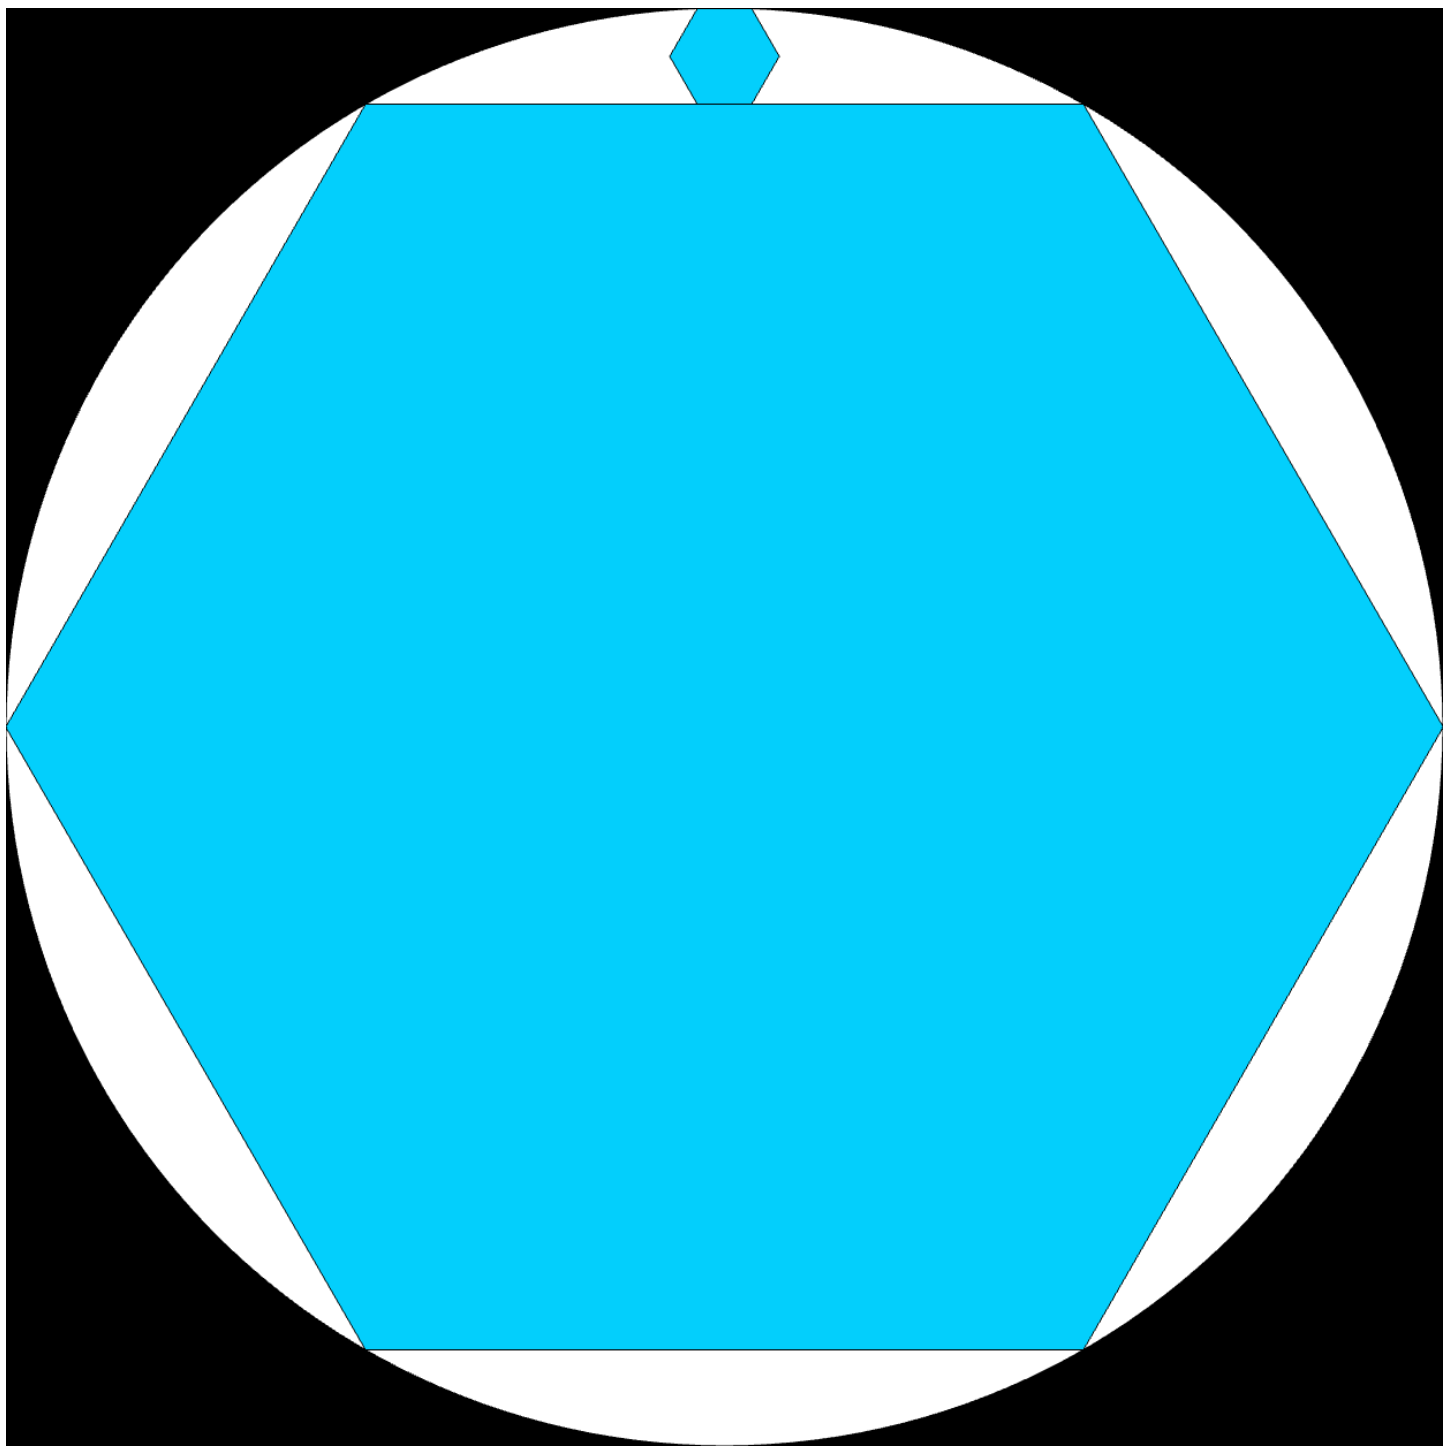
\includegraphics[scale = 0.75]{EmbedHexagon.png}
	\caption{The larger hexagon has unit side length. The circle circumscribes the larger hexagon. The smaller hexagon has unknown length.}
	\label{fig:largerHexagon}
\end{figure}

\subsection*{Problem}

A regular hexagon with side length 1 is circumscribed by a circle. Another regular hexagon is placed so that one of its sides overlaps with the larger regular hexagon, and the pair of vertices on the opposite side lie on the circle. Figure $\ref{fig:largerHexagon}$ shows the setup just described. 

What is the side length of the smaller regular hexagon. 

\subsection*{Solution}

\begin{figure}[h]
	\centering
	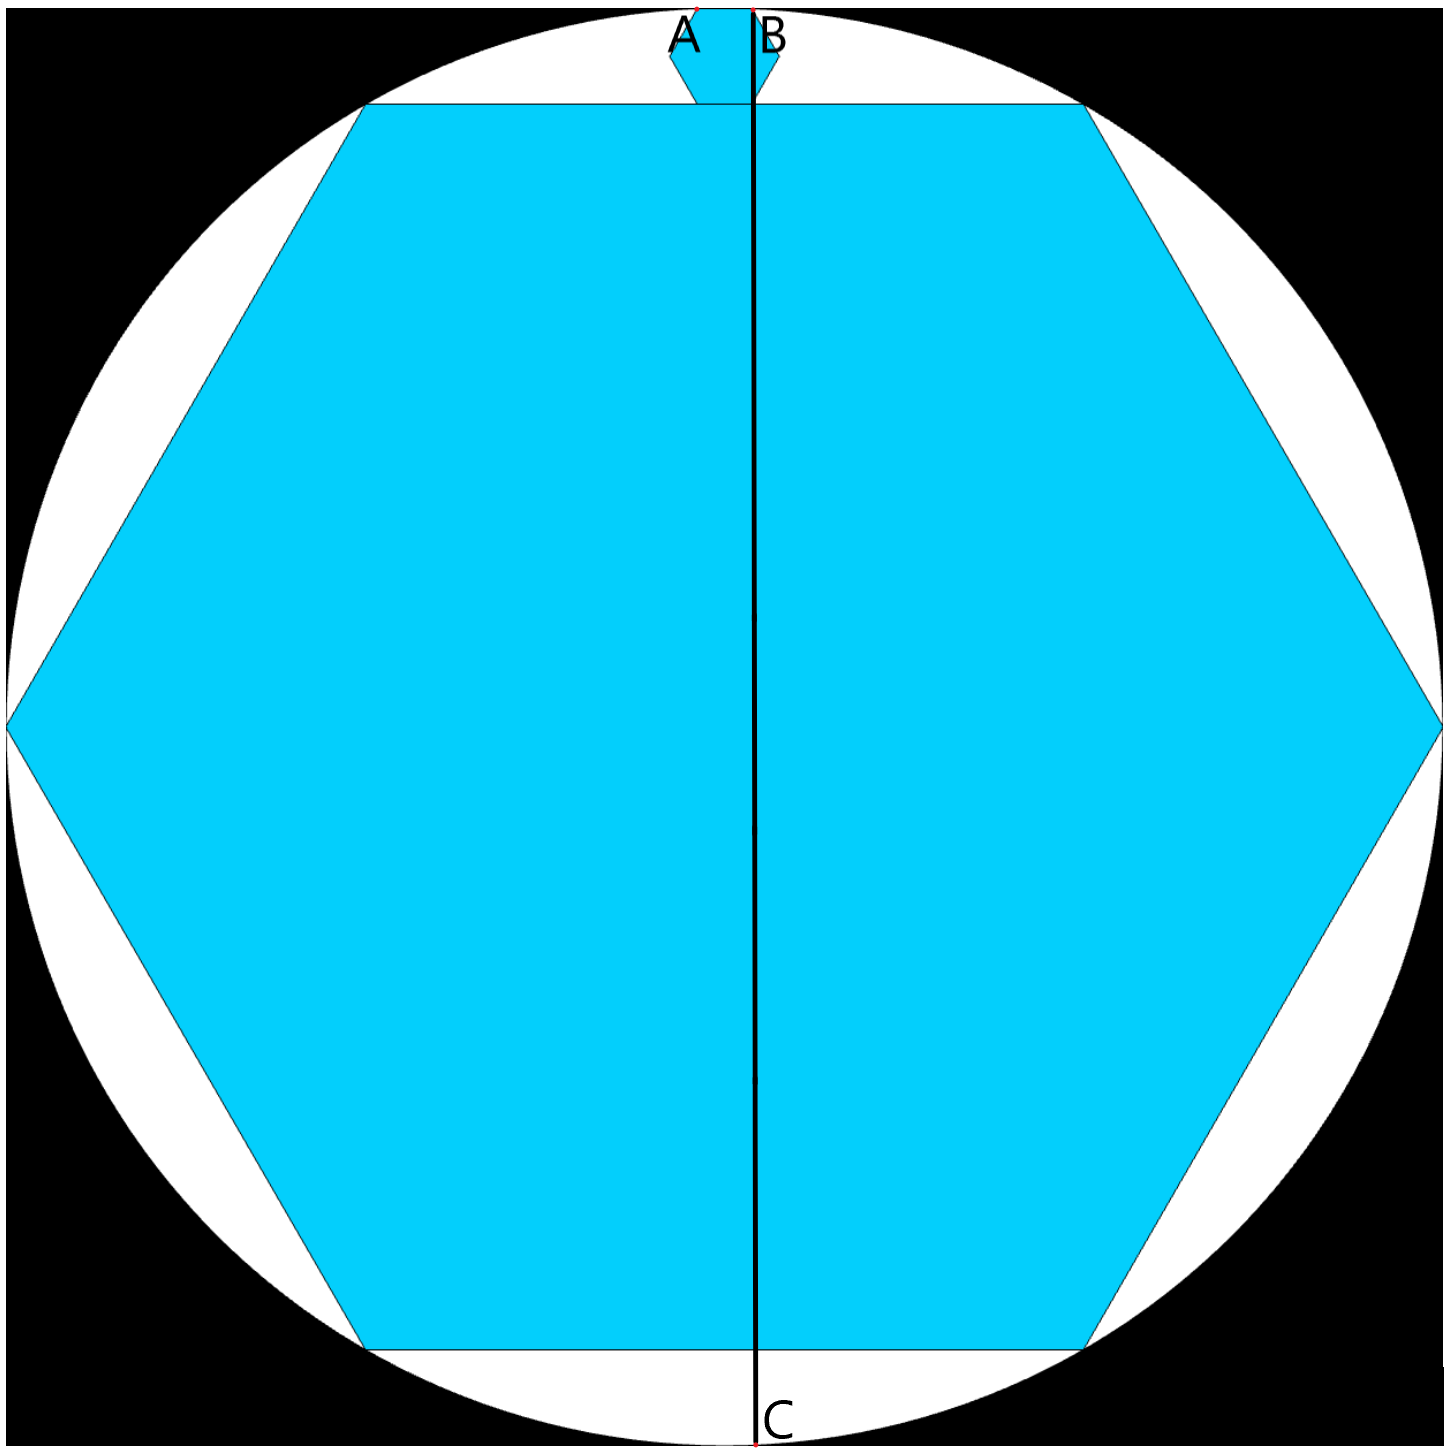
\includegraphics[scale = 0.25]{LinedHexagon.png}
	\caption{We construct a line that passes through two vertices of the smaller hexagon, shown in black above. We can then construct a right triangle $\triangle{\rm ABC}$, whose sides consist of the line just mentioned, the side of the smaller hexagon perpendicular to the black line, and a diameter of the circle.}
	\label{fig:triangleConstruction}
\end{figure}

In order to determine the side length of the smaller hexagon, we will construct a right triangle, whose sides can be determined from the dimensions of the two hexagons. 

We could imagine flipping the setup in Fig. $\ref{fig:largerHexagon}$ horizontally across its center, so that the smaller hexagon lies on the bottom edge of the larger hexagon. The smaller hexagon would be the same whether it lies on the top or bottom edge, but we observe that the vertices of the top hexagon can be paired with the vertices of the bottom hexagon so that each pair defines a diameter of the circle. Concretely, point $C$ in Fig. $\ref{fig:triangleConstruction}$ can be chosen so that $AC$ is a diameter of the circle and $BC$ is a vertical line. 

If we denote the side length of the smaller hexagon by $a_1$, then we can draw conclusions about the lengths of several segments, $AB$, $AC$, and $BC$. As $AB$ is a side of the smaller hexagon, it must have length $a_1$. Since the side length of the larger hexagon is $a_0=1$, the circle has radius $1$. To illustrate this point, we could imagine the larger hexagon to be made up of six equilateral triangles. Thus, the circle's diameter has length 2. Each equilateral triangle has altitude $\sqrt{3}/2\cdot a_0$, and so we can see that the perpendicular distance between opposite sides of the larger hexagon is $\sqrt{3}$, and the smaller hexagon likewise has altitude $\sqrt{3} a_1$. By its construction, the line $BC$ has length equal to the sum of the larger hexagon's altitude and twice the smaller hexagon's altitude, i.e., $\overline{BC}=\sqrt{3}(1+2a_1)$. 

From its construction, triangle $\triangle{\rm ABC}$ is a right triangle, and so we can apply the Pythagorean theorem, 
\begin{align*}
2^2 &= a_1^2 + \left(\sqrt{3}(1+2a_1)\right)^2 \\
4 &= a_1^2 + 3(1+4a_1 + 4a_1^2) \\
0 &= 13 a_1^2 + 12 a_1 - 1 \\
0 &= (13a_1-1)(a_1+1)
\end{align*}  

It follows that $a_1 = 1/13$.

\subsection*{Extra credit}

For extra credit, we can ask for the side length of the even smaller hexagons stacked on top of the two hexagons already shown. See the \href{https://fivethirtyeight.com/features/can-you-design-the-perfect-wedding/}{problem animation} for a clearer picture. From their definition, it is clear that the same construction will work in both of these cases, with only minor differences. 

For the next smaller hexagon, with side length $a_2$, we can imagine the same inversion to define another right triangle, with hypotenuse 2 and side length $a_2$. Its third side is given by $2\sqrt{3}a_2+2\sqrt{3}a_1+\sqrt{3}a_0=\sqrt{3}(2a_2 + 15/13)$. Applying the Pythagorean theorem, we can write 
\begin{align*}
2^2 &= a_2^2 + \left( \sqrt{3}(2a_2 + 15/13) \right)^2 \\
0 &= 13 a_2^2 + 180a_2/13 - 1/169.
\end{align*}

Applying the quadratic formula, we have $a_2 = (\sqrt{8113}-90)/169$. 

For the smallest hexagon, with side length $a_3$, an analogous construction is possible to define a final right triangle, with hypotenuse 2 and side length $a_3$. Similar to the previous cases, its third side is the sum of altitudes for each hexagon through which it passes, i.e., $\sqrt{3}(2a_3+2a_2+2a_1+a_0)$, since it passes through the central hexagon once and each smaller hexagon on both the top and bottom. Applying Pythagorean theorem, we can write 
\begin{align*}
2^2 &= a_3^2 + 3(2a_3 + 2a_2 + 2/13+1)^2 \\
0 &= (2739997+30420\sqrt{8113})a_3^2 + (2920500+32424\sqrt{8113})a_3-1/13
\end{align*}

As before, we could apply the quadratic formula to determine $a_3$, 
\begin{align*}
a_3 &= \frac{1}{169}\frac{16213-180\sqrt{8113}}{90+12\sqrt{8113}+\sqrt{1387141-180\sqrt{8113}}}
\end{align*}

Approximating, $a_1 \approx 7\cdot 10^{-2}$, $a_2 \approx 4.3 \cdot 10^{-4}$, and $a_3 \approx 1.3 \cdot 10^{-8}$. Extrapolating somewhat, further hexagons seem to grow doubly exponentially smaller $a_n \approx 10^{-2^n}$, although this conclusion would certainly be reinforced by a few more data points. 




\end{document}